%TC: macro \marginfootnote [other]
%TC: envir SCfigure [] other
%TC: macrocount beginSCfigure [figure]
\documentclass[11pt]{report}
\usepackage{preamble}
\setcounter{chapter}{4}
\graphicspath{{../img/}}

\externaldocument{morphometric-framework}

\begin{document}
\chapter{Applications of morphometric correlations: local structure in the hard sphere liquid}
\epigraph{\textbf{hardball 1.1} \emph{informal} Uncompromising and ruthless methods or dealings.}{Oxford English Dictionary}

\section{Introduction}

We wish to describe local structure.
Ultimately, we wish to learn about the structure of the energy landscape in hard spheres.
To do so we must characterise the main features of the landscape, namely the different geometric packings and assign weights (free energies) to them.
This is a worthy goal in its own right, perhaps not that interesting for hard spheres but useful for wider applications (e.g.\ predicting self assembly, guiding chemical synthesis, understanding protein folding kinetics and predicting the native state and design).

The path we take is as follows:
\begin{enumerate}
\item We need some means of weighting points in the energy landscape: we do this using the morphometric approach (cf previous chapter)
\item A means of characterising and approximating the entire phase space: energy landscape formalism (next). This has two subgoals:
  \begin{enumerate}
  \item Divide the landscape into stationary points: minima and saddles.
    These stationary points characterise submanifolds of the entire landscape, \emph{basins} in the case of minima and \emph{reaction paths} in the case of saddles.
  \item Integrate over connected manifolds with weight function (potential of mean force) to obtain their free energies.
  \end{enumerate}
\end{enumerate}

%Another way of saying this is we need an integrand and boundary conditions.

\subsection{Connection with energy landscape descriptions}

\begin{itemize}
  \item First describe the energy landscape description.
  \item Based on low-temperature expansion arguments.
  \item Mean-field: Laplace method/saddle-point.
  \item Gaussian expansion around this result (called Harmonic approximation in energy landscape/chemistry literature).
\end{itemize}

\begin{SCfigure}[H]
  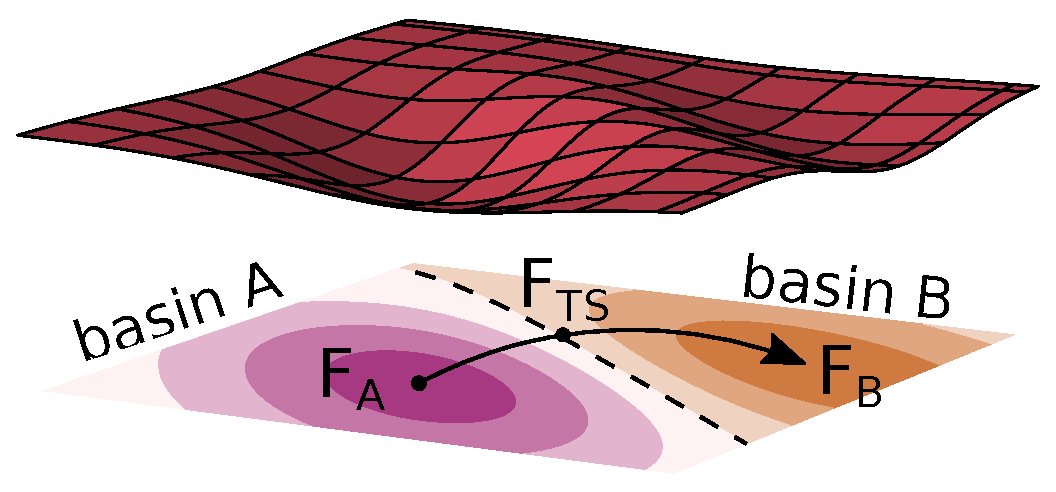
\includegraphics[width=\linewidth]{toy-landscape}
  \caption{A cartoon energy landscape for a 2-dimensional phase space.
    The landscape features two local minima: $A$ and $B$.
    The area surrounding each minima defines its basin: any point from which the minima can be found by moving downhill belongs to the basin.}
\end{SCfigure}

In the case of local arrangements of hard spheres, rigid packings seem to correspond to minima of the potential of mean force.
I cannot prove this for the case of morphometric approach, but I cannot find a counter example.
Possibly can prove they are minimal volume.

\section{Locally favoured structures in hard spheres}

\subsection{Concentrations of local structure}

How do we define a local structure?
Most of the literature on structure in amorphous systems falls into one of either two categories
Almost all methods for Common methods:
\begin{itemize}
  \item Bond orientational order parameters
  \item Bond networks: take some bond detection algorithm (voronoi, 
Fom the partition function of the potential of mean force
Suppose we have a definition of a
\end{itemize}

From the definition of the probability density function in Eq.\ \eqref{eq:n-density-pdf}, the total number of local structures of a particular type in a volume $V$ is
\begin{equation}\label{eq:structure-population}
  \mathcal{N} =
  \int_{\mathcal{Q}} \rho^n g^{(n)}(\vec{r}^n) \, d\vec{r}^n,
\end{equation}
where $\mathcal{Q}$ is the domain \emph{defining} the local structure.
To get the free energy expression used in the main text we consider the manifold diffeomorphic to translations, defining $\mathcal{Q} = \mathcal{D} \rtimes \mathbb{V}$ where $\mathbb{V}\subset \mathbb{R}^3$ is the system volume.
Exploiting translational invariance of the potential of mean force, we fix one particle at the origin and integrate the center of mass over the system volume giving
\begin{equation}
  \mathcal{N} =
  \rho^n V \int_{\mathcal{D}} g^{(n)}(\vec{r}^n) \, d\vec{r}^{n-1}.
\end{equation}
We defined a free energy by taking $\mathcal{N} = \sigma^{3(n-1)} \rho^n V e^{-\beta F}$, which together with the above expression gives Eq.\ \eqref{eq:local-structure-free-energy} in the main text.

More generally, we consider the manifold diffeomorphic to translations \emph{and} rotations.
We define $\mathcal{Q} = \mathcal{D}' \rtimes SE(3)$ where $\textrm{SE}(d)$ is the $d$-dimensional special Euclidean group, leaving the $\mathcal{D}'$ as the space of the structure's internal motion.
We separate rigid body from internal motion by applying the following transformation to each particle coordinate
\begin{equation}
  \vec{r}(\{\vec{t}, \vec{\theta}, \vec{x}\}) =
  \vec{t} + \vec{R}(\vec{\theta}) \cdot \vec{q}(\vec{x}),
\end{equation}
where $\vec{t}$ is the translation vector, $\vec{\theta}$ the Euler angles, $\vec{R}$ the rotation matrix, and $\vec{x} \in \mathbb{R}^{3n-6}$ represents the internal coordinates.
We need to compute the metric of this transformation $G_{ij} = \vec{G}_i \vec{G}_i^T$ where the (generally curvilinear) basis vectors are $\vec{G}_i = \partial_i \vec{r}$.
To simplify calculation we choose $\vec{q}(\vec{x})$ to always be in the center-of-mass frame and orthogonal to rotations such that $G_{ij}$ reduces to block-diagonal form.
If the rotation matrix is expressed in Euler-angle representation as $\vec{R}(\vec{\theta}) = \vec{R}_3(\theta_3) \vec{R}_2(\theta_2) \vec{R}_1(\theta_1)$ then we have%
\marginfootnote{While the final form of $\vec{G}$ is elegant, I do not have a straightforward way of getting it; it involved a lot of guesswork and within Mathematica to find a form of $\vec{U}$ which gives the middle block.
  There is probably a more direct route.}
\begin{equation}
  G_{ij}(\{\theta_i\}, \vec{x}) =
  \begin{pmatrix}
    n \vec{E} & 0 & 0 \\
    0 & \vec{U}^T(\vec{\theta}) \vec{I}(\vec{x}) \vec{U}(\vec{\theta}) & 0 \\
    0 & 0 & \overline{G_{ij}}(\vec{x})
  \end{pmatrix},
\end{equation}
where $\vec{E}$ is the identity matrix, $\overline{G_{ij}}$ is the metric for internal motion, and we have defined the matrix $\vec{U}$ as
\begin{equation}
  \vec{U}(\vec{\theta}) =
  \begin{pmatrix}
    1 &  0              & -\sin{\theta_2} \\
    0 &  \cos{\theta_1} &  \cos{\theta_2} \sin{\theta_1} \\
    0 & -\sin{\theta_1} &  \cos{\theta_2} \cos{\theta_1} \\
  \end{pmatrix}
  \qquad
  \begin{aligned}
    \theta_1 &\in [0,2\pi] \\
    \theta_2 &\in \left[-\frac{\pi}{2},\frac{\pi}{2}\right] \\
    \theta_3 &\in [0,2\pi].
  \end{aligned}
\end{equation}
Note $\det{\vec{U}} = \cos{\theta_2}$.
The volume element in the new coordinates is
\begin{equation}
  d\vec{r}^n = \frac{\sqrt{\det G_{ij}(\vec{x})}}{\nu}
  \, d^3 \vec{t} \, d^3 \vec{\theta} \, d^{3n-6} \vec{x},
\end{equation}
where $\nu$ is the symmetry number (discussed below) and
\begin{equation}
  \sqrt{\det G_{ij}(\vec{x})} =
  \cos{\theta_2} \sqrt{\det{\vec{I}(\vec{x})}}
  \sqrt{n^3 \det{\overline{G_{ij}}(\vec{x})}}.
\end{equation}
The symmetry number emerges as the choice of internal coordinates typically fixes the particle labels breaking permutation symmetry; we have to multiply by the $n!$ possible labellings, which introduces double counting if the structure possesses rotational symmetry so we have to divide by the correcting factor $\nu$.
This is explained in detail in Ref.\ \cite{Cates2015}.
Thus \eqref{eq:structure-population} reduces to
\begin{equation}\label{eq:structural-partition-function-detailed}
  \frac{\mathcal{N}}{\rho^n V}
  =
  \frac{8\pi^2 \sqrt{n^3}}{\nu} \int_{D'}
  g^{(n)}(\vec{x}) \,
  \sqrt{\det{\overline{G_{ij}}(\vec{x})} \det{\vec{I}(\vec{x})}}
  \, d^{3n-6} \vec{x}.
\end{equation}
Note that in the limit of linear molecules, i.e.\ where all particles fall on a line, the above approach fails as there is one less rotation mode requiring a modified description.

In general, the integrand in \eqref{eq:structural-partition-function-detailed} is only exactly solvable for the simplest geometries due to the high dimensionality of $\vec{x}$.
This is further complicated by the fact that the basis vectors for $\overline{G_{ij}}$ are curvilinear.
We use two methods for evaluating these integrands:
\begin{enumerate}
\item Monte Carlo simulation: described in the next section.
\item Analytically via perturbation theory: described in sections \ref{SI:bond-distance} and \ref{SI:reaction-path}.
  We use this for a similar integrand along a reaction path where Monte-Carlo cannot be used directly.
\end{enumerate}

\subsection{Bond-distance space}
To evaluate the integrand in Eq.\ \eqref{eq:structural-partition-function-detailed} analytically we need to choose a representation for $\vec{x}$ which is diffeomorphic to $\vec{r}^n$.
For \emph{minimally constrained geometries}, i.e.\ structures with exactly $3n-6$ contacts, a convenient representation exists: bond distance space.
Following Ref.\ \cite{Holmes-Cerfon2013} and its accompanying Supplementary Information we choose each element of $\vec{x}$ to represent the distances between particles in contact, where contact occurs at $\vec{x} = (\sigma, \dots, \sigma)$.
Thus increasing elements of $\vec{x}$ corresponds to thermal fluctuations away from contact.
This representation naturally expresses the limits of integration given in the main text as $\sigma \le x_i \le \sigma_{cut}$.

To evaluate the integral we need expressions for the internal metric and moment of inertia terms.
The internal metric is defined in terms of the Jacobian matrix $\vec{J} \in \mathbb{R}^{3n \times 3n-6}$
\begin{equation}
  \overline{G_{ij}} = \vec{J}^T \vec{J}
\end{equation}
where the matrix entries are given by
\begin{equation}
  J_{ij} = \frac{\partial q_i}{\partial y_j}.
\end{equation}
In practice it is easier to calculate its inverse numerically (via finite differences) using
\begin{equation}
  J_{ij}^{-1}
  = \frac{\partial y_j}{\partial q_i}
  = \left. \frac{\partial y_j}{\partial x_i}
  \right|_{\vec{\theta} = \vec{t} = \vec{0}}
\end{equation}
which has linearly independent rows for a minimally constrained geometry so we recover $\vec{J}$ from $\vec{K} = \vec{J}^{-1}$ using the matrix inversion formula $\vec{J} = (\vec{K}^T\vec{K})^{-1} \vec{K}^T$.
The above expressions all depend implicitly on the point $\vec{x}$ as the coordinate scheme is curvilinear, so to keep the integral tractable we approximate this to leading order as
\begin{equation}
  \sqrt{\overline{G_{ij}}(\vec{x})} \simeq \sqrt{\overline{G_{ij}}(\vec{x}_0)}
\end{equation}
where $\vec{x}_0 = (\sigma,\dots,\sigma)$ is contact.
Thus the integral becomes
\begin{equation}\label{eq:structural-partition-function-approximated}
  \frac{\mathcal{N}}{\rho^n V}
  =
  \frac{8\pi^2 G_0}{\nu} \int_{D'}
  g^{(n)}(\vec{x}) \,
  \sqrt{\det{\vec{I}(\vec{x})}}
  \, d^{3n-6} \vec{x}
\end{equation}
where $G_0 = \sqrt{n^3 \det{\overline{G_{ij}}(\vec{x}_0)}}$.

Finally, we write the distribution function in terms of the potential of mean force and expand this and the moment of inertia to first order, as in
\begin{align}
  \phi^{(n)}(\vec{x}) &=
  \phi^{(n)}(\vec{x}_0) +
  (\vec{x} - \vec{x}_0) \cdot
  \left. \vec{\nabla} \phi^{(n)}(\vec{x}) \right|_{\vec{x} = \vec{x}_0} +
  \mathcal{O}(\vec{x}^2), \\
  \sqrt{\det{\vec{I}(\vec{x})}} &=
  \sqrt{\det{\vec{I}(\vec{x}_0)}} +
  (\vec{x} - \vec{x}_0) \cdot
  \left. \vec{\nabla} \sqrt{\det{\vec{I}(\vec{x})}} \right|_{\vec{x} = \vec{x}_0} +
  \mathcal{O}(\vec{x}^2).
\end{align}
Using the analytical gradient expressions given in Section \ref{SI:line-curvature} makes this calculation very efficient.
The integral \eqref{eq:structural-partition-function-approximated} separates into $3n-6$ independent one-dimensional integrals of the form
\begin{equation*}
  \int_\sigma^{\sigma_{cut}} (a_i + b_i x_i) e^{-c_i x_i} dx_i
  = \left[
    - \left(
    \frac{(a + b_i x_i)}{c_i} + \frac{b_i}{c_i^2} \right) e^{-c_i x_i}
  \right]_\sigma^{\sigma_{cut}},
\end{equation*}
where $a_i$, $b_i$ and $c_i$ are constants.

Loosely speaking, this is the hard-particle analogue of the harmonic approximation with the difference here being that the first derivative does not vanish at the minimum.
For $n=6$ this expansion works rather well, as all structures have exactly $3n-6$ bonds and this perturbation theory captures the free energy well when compared with the ``exact'' result from thermodynamic integration.

\subsection{Worked examples}
Where the partion function is sufficiently simple that we can perform the integral analytically

\subsubsection{$n = 2$ (the coordination shell or dimer)}

We have the average number neighbours less than some distance $r$.
\todo{Comment on connection between this expression and the more general form which uses the moment of inertia as the metric.}
\begin{equation}
  z(r) = 4\pi \int_0^r r^2 g^{(2)}(r) dr
  = 4\pi e^{2\beta \mu^{ex}} \int_1^r r^2 e^{-\beta \Delta \Omega(r)} dr
\end{equation}
This is a common measurement where $r$ is taken up to the first minimum of the $g(r)$ then $z$ corresponds to the number in the ``first-shell'' (i.e. the coordination number).

\subsubsection{$n = 3$}
Average concentration of triangles
\subsection{Monte-Carlo algorithm for $n > 3$}
\subsection{$n \le 13$ results}
For selected structures we compare the concentrations of local structures from theory against molecular dynamics simulations.
This confirms that the theory accurately predicts concentrations of many-particle local structures within the hard sphere liquid.
\subsection{Density of states for all hard sphere packings $n \le 14$}
From theory, and how this is affected by changes in density

\section{Dynamical barriers along reaction paths in hard spheres}
\subsection{Free energy along a reaction path in hard spheres}
\subsubsection{Perturbation theory: alternative to harmonic approximation for hard potentials}
\subsection{Scaling of dynamical barriers with volume fraction}
\subsubsection{Worked example $n = 6$}
Simplest accessible reaction path: transition between the $n = 6$ tripyramid and octahedron.
\subsubsection{Reaction paths for $7 \le n \le 14$}

\section{Nucleation of the crystal in hard spheres}

\end{document}
